\begin{figure}
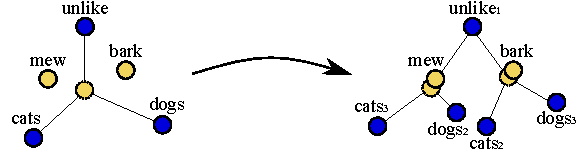
\includegraphics{positional-model}
\caption
  [Training objective of the positional language model]%
  {In the general and subword models, sentences such as
   ``Unlike dogs, cats mew'' and ``Unlike cats, dogs bark''
   would pull the input vectors (blue) in the opposite directions.  In the
   positional model, the input vectors are weighted by positional vectors
   and can satisfy both sentences.}
\label{fig:positional-model}
\end{figure}
